\section{Plan de développement}
    \begin{frame}{Plan de développement}{Introduction}
      Introduction PDD...
    \end{frame}
  \subsection{Diagramme de Gantt}
    \begin{frame}{Plan de développement}{Diagramme de Gantt}
      \begin{figure}[!h]
          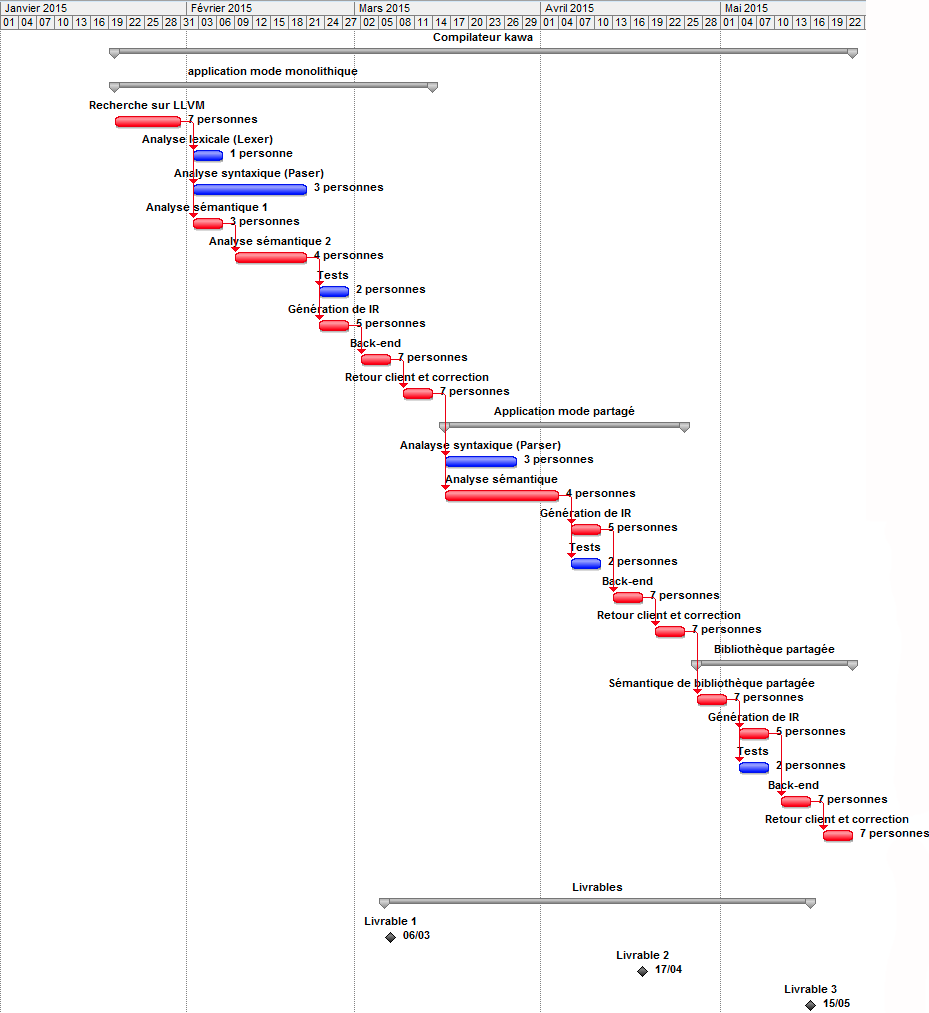
\includegraphics[width=7cm]{../pdd/fig/decoupage_cycles.png}
          \caption{Decoupage général en cycles.}
          \label{decoupage_cycles}
        \end{figure}
    \end{frame}
  \subsection{Stratégie de livraison en itérations}
    \begin{frame}{Plan de développement}{Stratégie de livraison en itérations}
      \begin{block}{Itération 1: Application en mode monolitique}
        
           \begin{itemize}
             \item<1-> Livraison le 06/03/2015
             \item<2-> Contenu: 
              \begin{itemize}
                \item<3-> Héritage.
                \item<4-> Polymorphisme.
              \end{itemize}
           \end{itemize}
        
      \end{block}
    \end{frame}
    %%%%
    \begin{frame}{Plan de développement}{Stratégie de livraison en itérations}
      \begin{block}{Itération 2: Application en mode partagé}
       
           \begin{itemize}
             \item<1-> Livraison le 17/04/2015
             \item<2-> Contenu:
              \begin{itemize}
                \item<3-> Héritage.
                \item<4-> Polymorphisme.
                \item<5-> Contrôle de typage.
              \end{itemize}
           \end{itemize}
        
      \end{block}
    \end{frame}
    %%%%
    \begin{frame}{Plan de développement}{Stratégie de livraison en itérations}
      \begin{block}{Itération 3: Livraison finale}
       
           \begin{itemize}
             \item<1-> Livraison le 15/05/2015
             \item<2-> Contenu: 
              \begin{itemize}
                \item<3-> Compilation en mode monolitique.
                \item<4-> Compilation d'application en mode partagé.
                \item<5-> Compilation de bibliothèque partagée.
              \end{itemize}
           \end{itemize}
        
      \end{block}
    \end{frame}
%%%%%%%%%%%%%%%%